
\newcommand{\printfigGraphTypes}{
    \begin{figure}
        \begin{subfigure}{.5\textwidth}
            \centering
            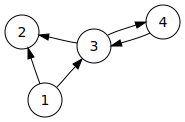
\includegraphics[width=.8\linewidth]{assets/images/Directed_graph_no_background.svg.pdf}
            \caption{Directed graph with cycle between nodes three and four.}
            \label{fig:directedgraph}
        \end{subfigure}
        \begin{subfigure}{.5\textwidth}
            \centering
            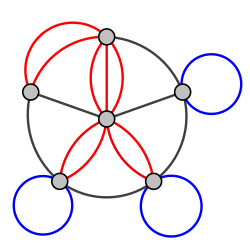
\includegraphics[width=.8\linewidth]{assets/images/Multi-pseudograph.svg.pdf}
            \caption{Multigraph with parallel edges and self-loops}
            \label{fig:multigraph}
        \end{subfigure}%
        \caption[]{Examples of first order graph symantics supported by Jaseci.\footnotemark}
        \label{fig:graph_examples}
    \end{figure}
    \footnotetext{Images credits to wiki contributers~\cite{wiki:Directed_graph_no_background.svg,wiki:Multi-pseudograph.svg}}
}


\newcommand{\printfigHelloWorldBaby}{
    \begin{figure}%{r}{0.5\textwidth}
        \centering
        \includegraphics[width=.3\linewidth]{assets/images/hello_world_baby.jpg}
        \caption[]{World's youngest coder with valid HTML on shirt.\footnotemark}
        \label{fig:hello_baby}
    \end{figure}
    \footnotetext{Image credit to wiki contributer~\cite{wiki:hello_world_baby.jpg}}
}

\newcommand{\printtabPrecedence}{
    \begin{table}[t]
        \footnotesize
        \centering
        \begin{tabular}{l l l}
            \toprule
            \textbf{Rank} & \textbf{Symbol}                            & \textbf{Description}                           \\
            \midrule
            1             & \texttt{( ), [ ], ., ::, spawn}            & Parenthetical/grouping, node/edge manipulation \\
            2             & \texttt{\textasciicircum, []}              & Exponent,  Index                               \\
            3             & \texttt{*, /, \%  }                        & Multiplication, division, modulo               \\
            4             & \texttt{+, -}                              & Addition, subtraction                          \\
            5             & \texttt{==, !=, >=, <=, >, <, in, not in } & Comparison                                     \\
            6             & \texttt{\&\&, ||, and, or  }               & Logical                                        \\
            7             & \texttt{-->, <--, -[]->, <-[]-}            & Connect                                        \\
            8             & \texttt{=, +=, -=, *=, /=, := }            & Assignment                                     \\
            \bottomrule
        \end{tabular}
        \caption{Precedence of operations in Jac}
        \label{tab:jacprecedence} % Unique label used for referencing the table in-text
        %\addcontentsline{toc}{table}{Table \ref{tab:jacprecedence}} % Uncomment to add the table to the table of contents
    \end{table}
}